
\section{Motivation}
\label{sec:motivation}

Peter Deutsch begins his classic list of ``Fallacies of Distributed
Computing'' with two concerns fundamental to distributed database
systems: ``\textit{1.)}  The network is reliable. \textit{2.)} Latency
is zero''~\cite{fallacies-deutsch}. On a single server, communication
channels are robust and relatively fast, and few single-server systems
need to account for a possibility of partial system failure. However,
in a distributed setting, both of these assumptions are no longer
valid. To extend Jim Gray's storage latency analogy, if memory is 1.5
hours from the CPU and disk is 2 years away, then, especially across
wide-area networks (WANs), remote server accesses can exceed 30 years,
with the added concern that messages can be lost in transit or delayed
indefinitely by network partitions~\cite{gray-rules}. Accordingly,
ignoring network failures and latency can ``cause big trouble and
painful learning experiences''~\cite{fallacies-deutsch}.

In this section, we quantify the effect of network partitions and
latency in several real-world deployments. While the importance of
network behavior is a topic of considerable speculation within the
database community~\cite{stonebraker2010errors}, there is mounting
evidence---both anecdotal and experimental---that partitions occur and
network latencies are non-negligible. We subsequently discuss the
impact of these findings on modern database operation and motivate the
case for HATs.

\subsection{Partitions in the Real World}

Network partitions---or, informally, communication link failures
between participants in a distributed system---are challenging. A
system facing network partitions faces the impossibility of
simultaneously maintaining a correct ``global'' view of system state
while simultaneously providing online operation to all of its
clients~\cite{davidson-survey}. For networks that do not partition,
maintaining semantic guarantees and available operation is
straightforward~\cite{stonebraker2010errors}. However, given the
\textit{possibility} of partitions, a system must be prepared to
either lose availability of operations or its ability to reason about
global state. In this section, we present evidence for the frequency
and non-triviality of WAN and LAN partitions.

According to James Hamilton, Vice President and Distinguished Engineer
on the Amazon Web Services team, ``network partitions should be rare
but net gear continues to cause more issues than it
should''~\cite{hamilton-partitions}. Anecdotal evidence confirms
Hamilton's assertion. In April 2011, a network misconfiguration led to
a twelve-hour long series of outages across the Amazon EC2 and RDS
services~\cite{amazon-netpartition}. Subsequent misconfigurations and
partial failures such as another EC2 outage in October 2012 have led
to full site disruptions for popular web services like Reddit,
Foursquare, and Heroku~\cite{ec2-downsites}. At a global scale,
hardware failures---like the 2011 outages in Internet backbones in
North America and Europe due a router
bug~\cite{juniper-partition}---and misconfigurations---such as BGP
faults in 2008~\cite{pakistan-youtube} and
2010~\cite{research-experiment-partition}---can cause widespread
partitions.

Many of our discussions with practitioners---especially those
operating on public cloud infrastructure---as well as reports from
large-scale operators like Google~\cite{dean-keynote} confirm that
partition management is an important consideration service operators
today. As an example of an actual system rearchitecture resulting from
partitions, less than one year after its announcement, Yahoo!'s PNUTS
developers explicitly added support for weaker, highly available
operation. The engineers explained that ``strict adherence [to strong
  consistency] leads to difficult situations under network
partitioning or server failures...in many circumstances, applications
need a relaxed approach''~\cite{pnuts-update}.

Several recent studies quantify partition behavior more rigorously. A
2011 study of several Microsoft datacenters found a mean of 40.8
network link failures per day (95th percentile: 136), with a median
time to repair of around five minutes (and up to one week). Perhaps
surprisingly, provisioning redundant networks only reduces impact of
failures by up to 40\%, meaning network providers cannot easily
curtail partition behavior~\cite{sigcomm-dc}. A 2010 study of over 200
wide-area routers found an average of 16.2--302.0 failures per link
per year with an average annual downtime of 24--497 minutes per link
per year (95th percentile at least 34 hours)~\cite{sigcomm-wan}. In
HP's managed enterprise networks, WAN, LAN, and connectivity problems
account for 28.1\% of all customer support tickets while 39\% of
tickets relate to network hardware.  The median incident duration for
highest priority tickets ranges from 114--188 minutes and up to a full
day for all tickets~\cite{turner2012failure}. Other studies confirm
these results, showing median time between failures over a WAN network
of approximately 3000 seconds with a median time to repair between 2
and 1000 seconds~\cite{ip-backbone-failures} as well as frequent path
routing failures on the Internet~\cite{labovitz-failures}. Isolating,
quantifying, and designing for these network failures is an area of
active research in networking
community~\cite{surviving-failures-bodik, uw-failure-networks}.

These results---which do not consider server-level failures (another
form of system partition that has also been studied at
scale~\cite{google-availability})---indicate that network partitions
\textit{do} occur within and across modern datacenters. We do not
intend to fixate on any particular statistical behavior but instead
observe that, as a general trend, partitions exist and must
accordingly be met with either unavailability at some servers or, as
we will discuss, relaxed semantic guarantees.

\subsection{Latency and Planet Earth}

Even with fault-free networks, distributed systems face the challenge
of communication latency, Deutsch's second ``Fallacy.'' In this
section, we quantify expected latencies, which are often
huge---hundreds of milliseconds---in a geo-replicated context.

Fundamentally, the speed at which two servers can communicate is
(according to modern physics) bounded by the speed of light. Two
servers located on opposite sides of the Earth face, in the best
case---communicating via a hypothetical link crossing through the
center of the planet---require a minimum 85.1 ms RTT (133.7 ms if sent
at ground level). As services are replicated to multiple,
geographically distinct sites, the cost of communication increases to
this upper bound.

In real deployments, latencies are actually higher than the speed of
light dictates due to routing, congestion, and processing times; if
not, servers a kilometer apart would enjoy a 6.7 $\mu$s RTT. To
illustrate the difference between intra-datacenter, inter-datacenter,
and inter-planetary networks, we performed a measurement study of
network behavior on Amazon's EC2, a widely-used public compute
cloud. We measured one week of ping times between all seven EC2
geographic ``regions'', across three ``availability zones'' (closely
co-located datacenters), and within a single ``availabilty zone''
(datacenter), at a granularity of 1s (dataset to be released).

We summarize the results of our network measurement study in
Table~\ref{table:rtt}. On average, inter-datacenter communication (1c)
is between 1.82 and 6.38 times faster than across geographically
co-located datacenters (1b) and between 40 and 647 times faster than
across geographically distributed datacenters (1a). The cost of
wide-area communication exceeds the speed of light: for example,
communicating from S\~{a}o Paulo to Singapore is lower-bounded by
speed-of-light transit RTT of 106.7ms but, on average, incurs a
362.8ms RTT (95th percentile: 649ms). As shown in
Figure~\ref{fig:rtt}, the distribution of latencies varies between
links, but the trend---in line with other recent studies~\cite{mdcc,
  redblue}---is clear: remote communication has a substantial cost.

\definecolor{min-lat-color}{HTML}{B2FF99}
\definecolor{max-lat-color}{HTML}{FF7F7F}

\begin{table}
\subfloat[Cross-region (OR:~Oregon, VA:~Virginia, TO:~Tokyo, IR:~Ireland, SY:~Sydney, SP:~S\~{a}o Paulo, SI:~Singapore)] {
  \begin{tabular}{|c|c|c|c|c|c|c|c|c|}
\hline
& \multicolumn{1}{c}{OR} & \multicolumn{1}{c}{VA} & \multicolumn{1}{c}{TO} & \multicolumn{1}{c}{IR} & \multicolumn{1}{c}{SY} & \multicolumn{1}{c}{SP} & \multicolumn{1}{c|}{SI} \\\hline
CA & \colorbox{min-lat-color}{22.5}   & 84.5   & 143.7   & 169.8   & 179.1   & 185.9   & 186.9  \\
OR &  & 82.9   & 135.1   & 170.6   & 200.6   & 207.8   & 234.4  \\
VA & &  & 202.4   & 107.9   & 265.6   & 163.4   & 253.5  \\
TO & & &  & 278.3   & 144.2   & 301.4   & 90.6  \\
IR & & & &  & 346.2   & 239.8   & 234.1  \\
SY & & & & &  & 333.6   & 243.1  \\
SP & & & & & &  & \colorbox{max-lat-color}{362.8}  \\
\hline
  \end{tabular}
}\vspace{.5em}

\subfloat[Across \texttt{us-east} AZs]{
  \makebox[.2\textwidth]{
    \begin{tabular}{|c|c|c|}\hline
 & \multicolumn{1}{c}{C} & \multicolumn{1}{c|}{D}\\\hline
B & \colorbox{min-lat-color}{1.08} & 3.12 \\
C & & \colorbox{max-lat-color}{3.57}  \\
\hline
  \end{tabular}}
 }
\subfloat[Within \texttt{us-east-a} AZ] {
  \makebox[.25\textwidth]{
  \begin{tabular}{|c|c|c|}\hline
 & \multicolumn{1}{c}{H2} & \multicolumn{1}{c|}{H3}\\\hline
H1  & 0.55   & \colorbox{max-lat-color}{0.56} \\
H2 &  & \colorbox{min-lat-color}{0.50}  \\
\hline
  \end{tabular}
 }}
\caption{Mean RTT times on EC2 (min and max highlighted)}
\label{table:rtt}
\end{table}

\begin{figure}
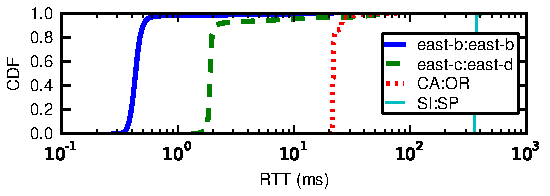
\includegraphics[width=\columnwidth]{graphs/ping-plot.pdf}
\caption{CDF of round-trip times for slowest inter- and intra-
  availability zone links compared to cross-region links.}
\label{fig:rtt}
\end{figure}


\subsection{CAP, Isolation, and Modern Systems}
\label{sec:modernacid}

Mitigating the effects of partitions and network latency is a
difficult task, requiring systems designers to choose between
fundamental trade-offs. In this section, we briefly discuss known
semantic limits for systems wishing to maintain high availability and
their impact on modern database systems. While the gold standard of
ACID semantics is unavailable, we show that many database systems
operate under much weaker models, motivating further study of these
models in a highly available context in the remainder of this paper.

One of the most popularly celebrated impossibility results in
distributed systems is Brewer's CAP Theorem, which, as formally proven
by Gilbert and Lynch, states that it is impossible to maintain
linearizability , or the ability to read the last completed write,
(``C,'' or ``consistency''---albeit poorly named) and replica
availability, or a guaranteed response, (``A'') in the presence of
network partitions (``P'')~\cite{gilbert-cap}. Brewer's Theorem has
roots in decades of distributed database
designs~\cite{davidson-survey} and has had a substantial impact on
recent large-scale distributed systems design: while CAP is narrowly
scoped to the impossibility of building highly available linearizable
systems, it is often interpreted to preclude a larger set of
guarantees, including ACID (transactional atomicity, consistency,
isolation and durability guarantees), as evidenced by the lack of
highly available systems providing them.

Database researchers and designers have long realized that
serializability---the gold standard of ACID isolation, which
guarantees application-level consistency---is not achievable in a
highly available system~\cite{davidson-survey}.  However, database
systems offer a range of ACID properties besides
serializability. Within a single-node database, the coordination
penalties associated with ensuring equivalence with a serial execution
can be severe and manifest themselves in the form of decreased
concurrency (and, subsequently, performance degradation, scalability
limitations, and, often, external aborts like
deadlocks)~\cite{gray-isolation}. Instead, databases offer a host of
so-called \textit{weak isolation} models that allow varying
restrictions on the space of schedules that are allowable by the
system~\cite{adya}. None of these weak isolation models guarantees
serializability, but the benefits of these models can often outweigh
costs of possible consistency anomalies that might arise from their
use.

To understand the prevalence of these weak isolation models, we
recently surveyed the default and maximum isolation models provided by
18 relational databases, often claiming to provide ``ACID'' or
``NewSQL'' functionality~\cite{hat-hotos}. As shown in
Table~\ref{table:existing}, only three out of 18 databases provided
serializability by default, and at least eight did not provide
serializability as an option at all. This is particularly surprising
when we consider the widespread deployment of many of these
non-serializable databases, like Oracle 11g, which are known to power
major businesses and product functionality. Given that these
transactional models are frequently used, our inability to provide
serializability in arbitrary HATs appears non-fatal for practical
applications. If application writers and database vendors have already
decided that the benefits of weak isolation outweigh potential
application inconsistencies, then, in a highly available environment
that prohibits serializability, similar decisions may be tenable.

\begin{table}
\begin{center}
\begin{small}
\begin{tabular}{|l|c|c|}
\hline
Database & Default & Maximum\\\hline
Actian Ingres 10.0/10S & S & S\\
Aerospike & RC & RC\\
Akiban Persistit & SI & SI\\
Clustrix CLX 4100 & RR & ?\\
Greenplum 4.1 & RC & S \\
IBM DB2 10 for z/OS & CS & S\\
IBM Informix 11.50 & Depends & RR\\
MySQL 5.6 & RR & S \\
MemSQL 1b & RC & RC\\
MS SQL Server 2012 & RC & S \\
NuoDB & CR & CR\\
Oracle 11g & RC & SI\\
Oracle Berkeley DB & S & S\\
Oracle Berkeley DB JE & RR & S\\
Postgres 9.2.2 & RC & S\\
SAP HANA & RC & SI\\
ScaleDB 1.02 & RC & RC\\
VoltDB & S & S\\
\hline
\multicolumn{3}{|p{7cm}|}{{\footnotesize RC: read committed, RR: repeatable read, SI: snapshot isolation, S: serializability, CS: cursor stability, CR: consistent read}}\\\hline

\end{tabular}
\caption{Default and maximum isolation levels for ACID and NewSQL
  databases as of January 2013 (from
  \protect\cite{hat-hotos}).}\vspace{-1.5em}
\label{table:existing}
\end{small}
\end{center}
\end{table}

The primary challenge in providing weak isolation in a HAT context is
that, unfortunately, it is unclear \textit{which} of these ACID
(particularly isolation) guarantees can be provided with high
availability. The existing algorithms for providing weak isolation are
typically designed for a single-node context and are, to the best of
our knowledge, unavailable due to a reliance on concurrency control
mechanisms like locking that are not resilient to partial failure
(Section~\ref{sec:evaluation}). Morever, we are not aware of any prior
literature that provides guidance as to the relationship between weak
isolation and high availability: prior work has examined the
relationship between serializability and high
availability~\cite{davidson-survey} and weak isolation on a
single-server~\cite{adya, ansicritique} but never weak isolation and
high availability taken together. We believe that this apparent gap in
the database literature is a possible contributing factor to the
often-apparent attitude~\cite{hn, foundation-article} that
general-purpose transactional semantics are either too expensive to
provide in many modern distributed databases---except under special
circumstances, such as providing operations over groups of co-located
data items~\cite{entitygroup}.
